
\documentclass[MaxHughesThesis.tex]{subfiles}

\begin{document}
\section{Motivation}
During the experiment, it was noticed that there was a disagreement between different values of the half-life.
As a side project and as a first chance to thoroughly investigate the data, a half-life analysis was made. 
These results have been published. % Give citation 
The previous measurements of the half-life of $^{20}$F are shown in figure \ref{fig:IDBefore}.

\begin{figure}[!htb]
	\centerline{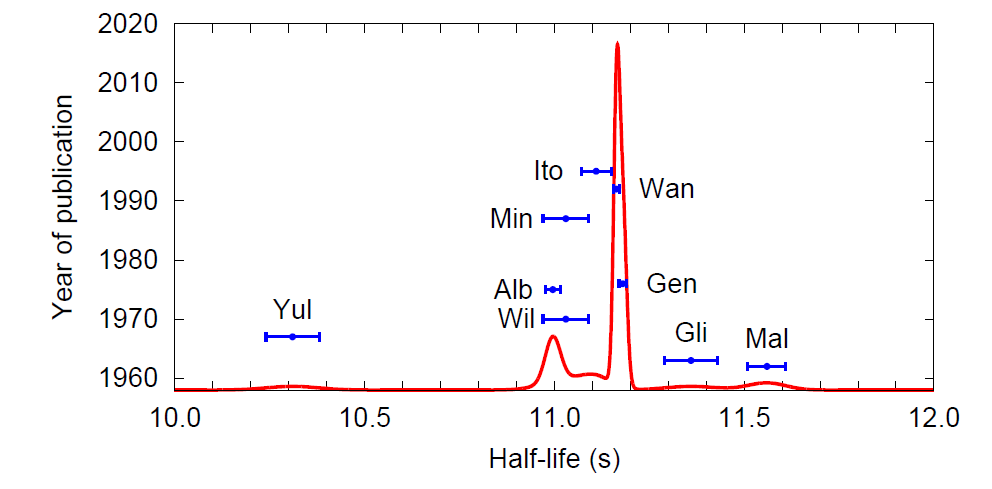
\includegraphics[width=0.78\textwidth]{fig_ideogramBefore.png}}
	\caption{Previous measurements of  the $^{20}$F half-life.
		 The labels correspond to: Mal~\cite{Mal62}, Gli~\cite{Gli63},
		Yul~\cite{Yul67}, Wil~\cite{Wil70}, Alb~\cite{Alb75}, Gen~\cite{Gen76},
		Min \cite{Min87}, Wan~\cite{Wan92} and Ito~\cite{Ito95}.}
	\label{fig:IDBefore}
\end{figure}

This ideogram has a red line which is a sum of Gaussian functions.
The centroids of the Gaussians are the central values of the measurements.
The sigmas are the errors, and each Gaussian is weighted by $\frac{1}{\sigma^{2}}$.
This is to see that there are two different values that the half-lives are converging to.


\section{Half life Data Analysis}
\label{sec:analysis}
First, the data was processed as described in the previous chapter.

\subsection{Data Selection}
Only the data from the PVT implantation set was used for the half-life analysis.
The PVT data was separated into 7 sets.
A summary of the set conditions is shown in table \ref{tab:ExpConditions}
As shown in the table, the major conditions were the PVT high voltage, the inhibitor box, and the beam current. 

%
\begin{table}[!hbt]
	\centering
	\caption{Settings for the PVT runs}
			\begin{tabularx}{\textwidth}{LRRRRRR}
			Set & Beam on Time [s] & Measuring Time [s] & PVT HV [v] & HV Inhibit Installed& Beam intensity [nA] & Runs \\ \hline
			1 & 1.67 & 30 & -975  & No & 30 & 9 \\		
			2 & 1.67 & 30 & -975  & No & 93 & 2 \\		
			3 & 1.67 & 30 & -975  & Yes & 30 & 9 \\		
			4 & 1.67 & 30 & -975  & Yes & 93 & 11 \\		
			5 & 1.67 & 30 & -856  & Yes & 30 & 93 \\		
			6 & 1.00 & 60 & -800  & Yes & 93 & 1 \\		
			7 & 1.10 & 20 & -780  & Yes & 93 & 10 	
			\end{tabularx}
			\label{tab:ExpConditions}
\end{table}
%

The inhibitor box was not installed until the third set of data. 
The inhibitor box reduced the high-voltage by about 100 V during the beam on period.
Without the box, the current on the PMT was saturated during the beam on period.
This caused a gain shift over time as the power supply recovered.
This time-dependent gain shift caused large systematic errors when the beta cuts were moved.
Thus, sets 1 and 2 where not used in the final analysis, but are listed here for completeness's sake.
These gain shifts can be seen in figure \ref{fig:pulserfig}.


\begin{figure}[!htb]
	\centerline{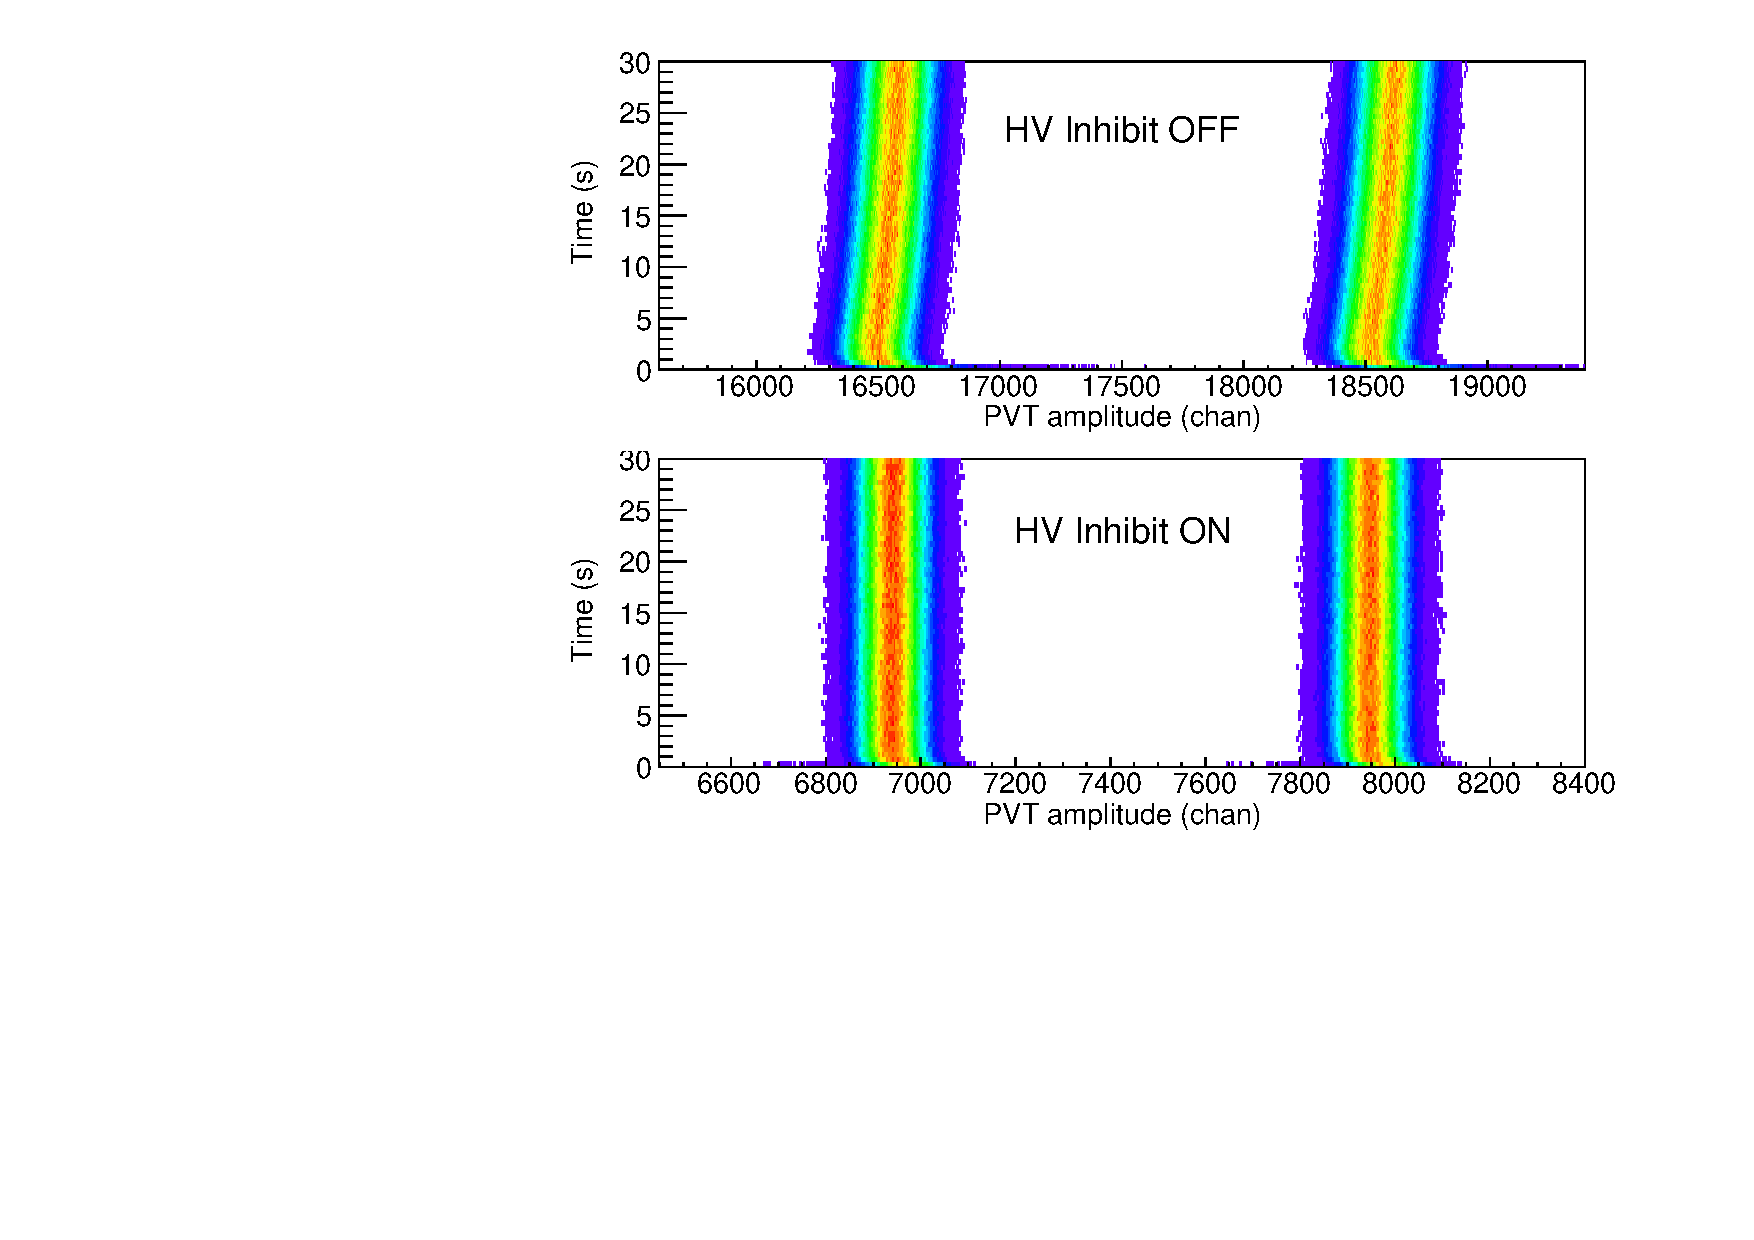
\includegraphics[width=0.78\textwidth]{fig_pulserVsTime.pdf}}
	\caption{The light pulse as a function of time for set 1.
		 The gain changes smoothly over time.
		 This causes a large change in the half-life as the beta cuts are moved.}
	\label{fig:pulserfig}
\end{figure}

\subsection{Cut Selection}
In order to do the half-life analysis, software coincidences were imposed.
Three conditions were set in total.
Two conditions were on the energy in the implantation detector and one of the four CsI(Na) detectors.
The gamma cuts are summarized in table \ref{tab:GammaCuts}.
An additional condition on the time difference between the events recorded in the two detectors. 
A sample spectrum of the gamma and beta energies is shown in figure \ref{fig:2DGraph}  

\begin{table}[!htb]
	\centering
	\caption{Energy cuts for the gamma detectors}
	\begin{tabular}{lrr}
	Detector & Lower Cut [ADC units] & Upper Cut [ADC units] \\ \hline
	Up & 1350 & 1650 \\
	Left & 1280 & 1600\\
	Down & 1440 & 1800 \\
	Right & 1450 & 1800
	\end{tabular}
	\label{tab:GammaCuts}
\end{table}

\begin{figure}[!htb]
	\centerline{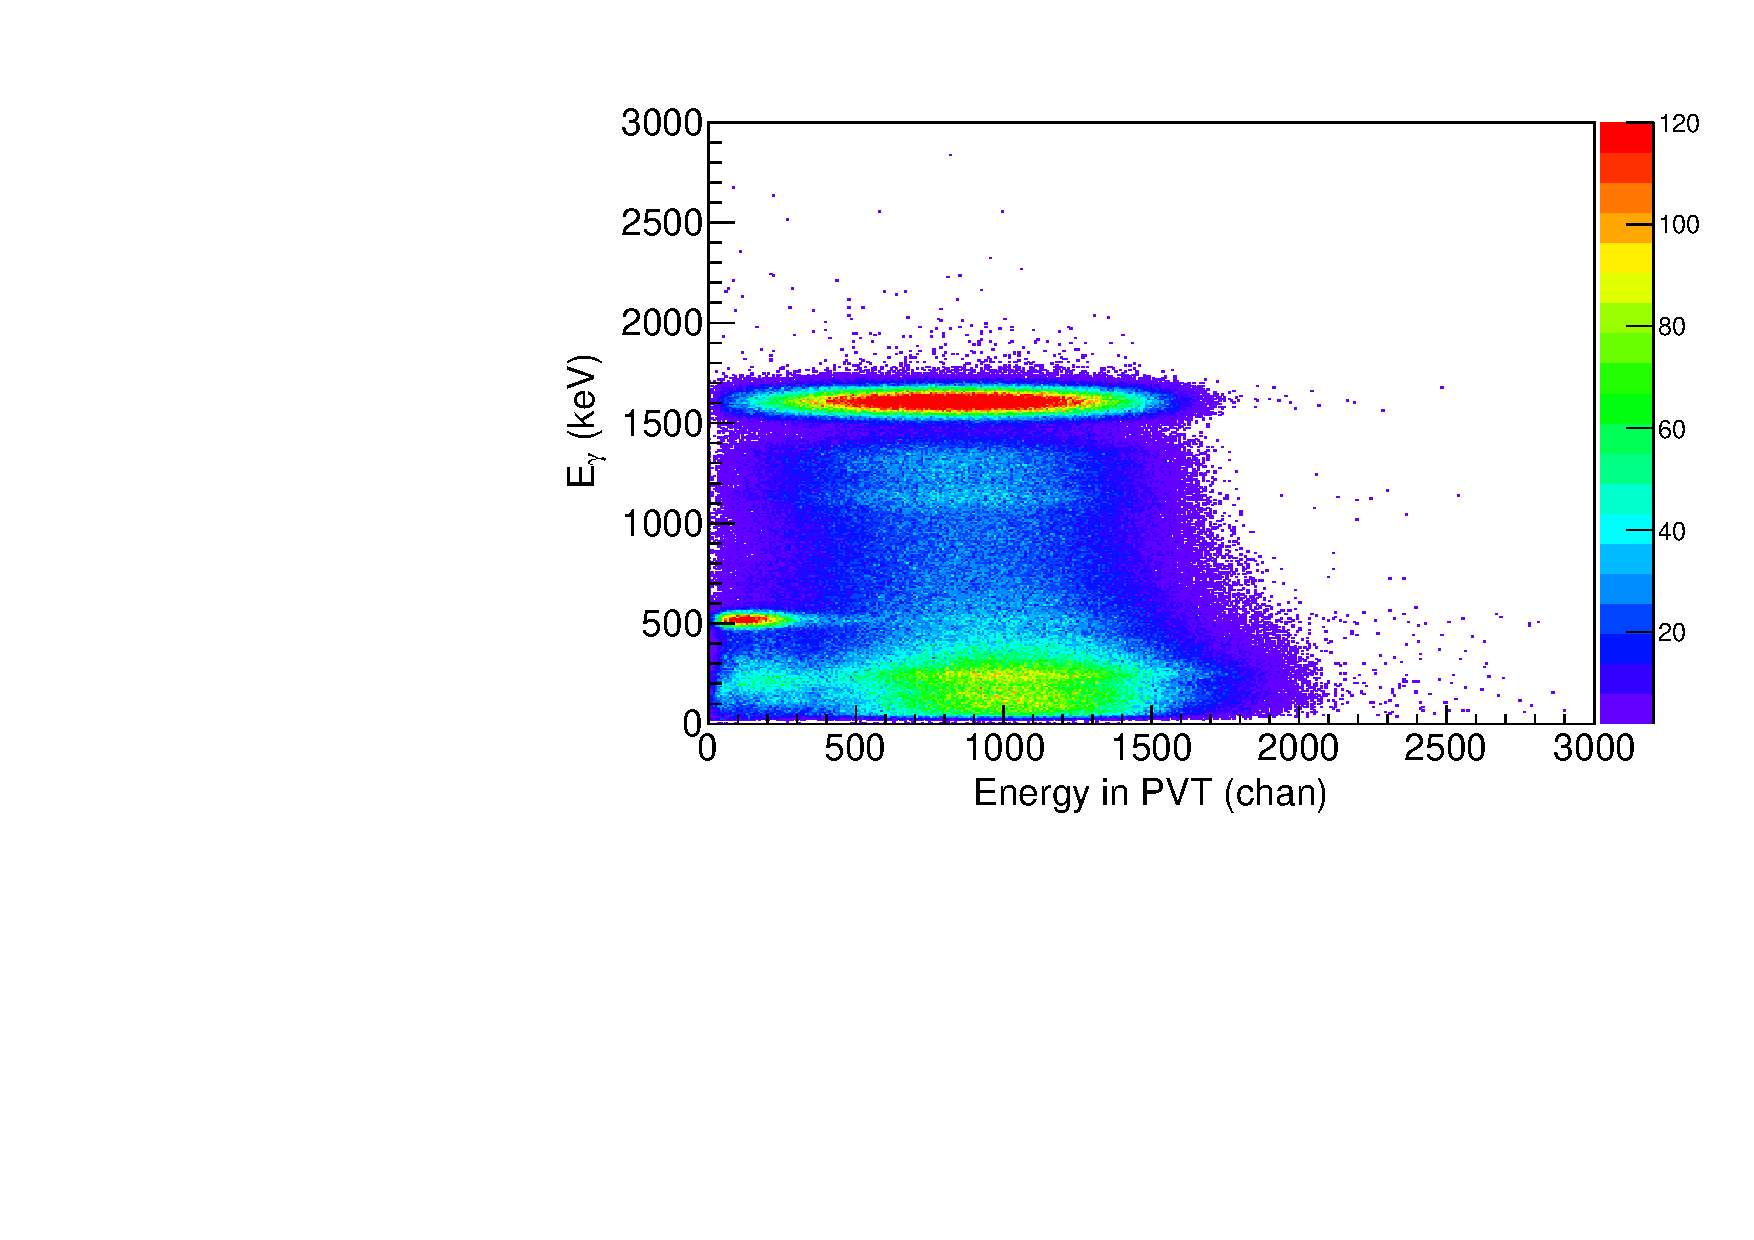
\includegraphics[width=0.78\textwidth]{fig_2Dh.pdf}}
	\caption{The $y$ axis shows the gamma detector energy.
		   The $x$ axis is the implant detector energy.
		   The $^{20}$F coincidence region can be seen towards the top of the spectrum.
		   The spectrum at 511 keV can be seen closer to the bottom of the figure.
		   }
	\label{fig:2DGraph}
\end{figure}

\begin{figure}[!htb]
	\centerline{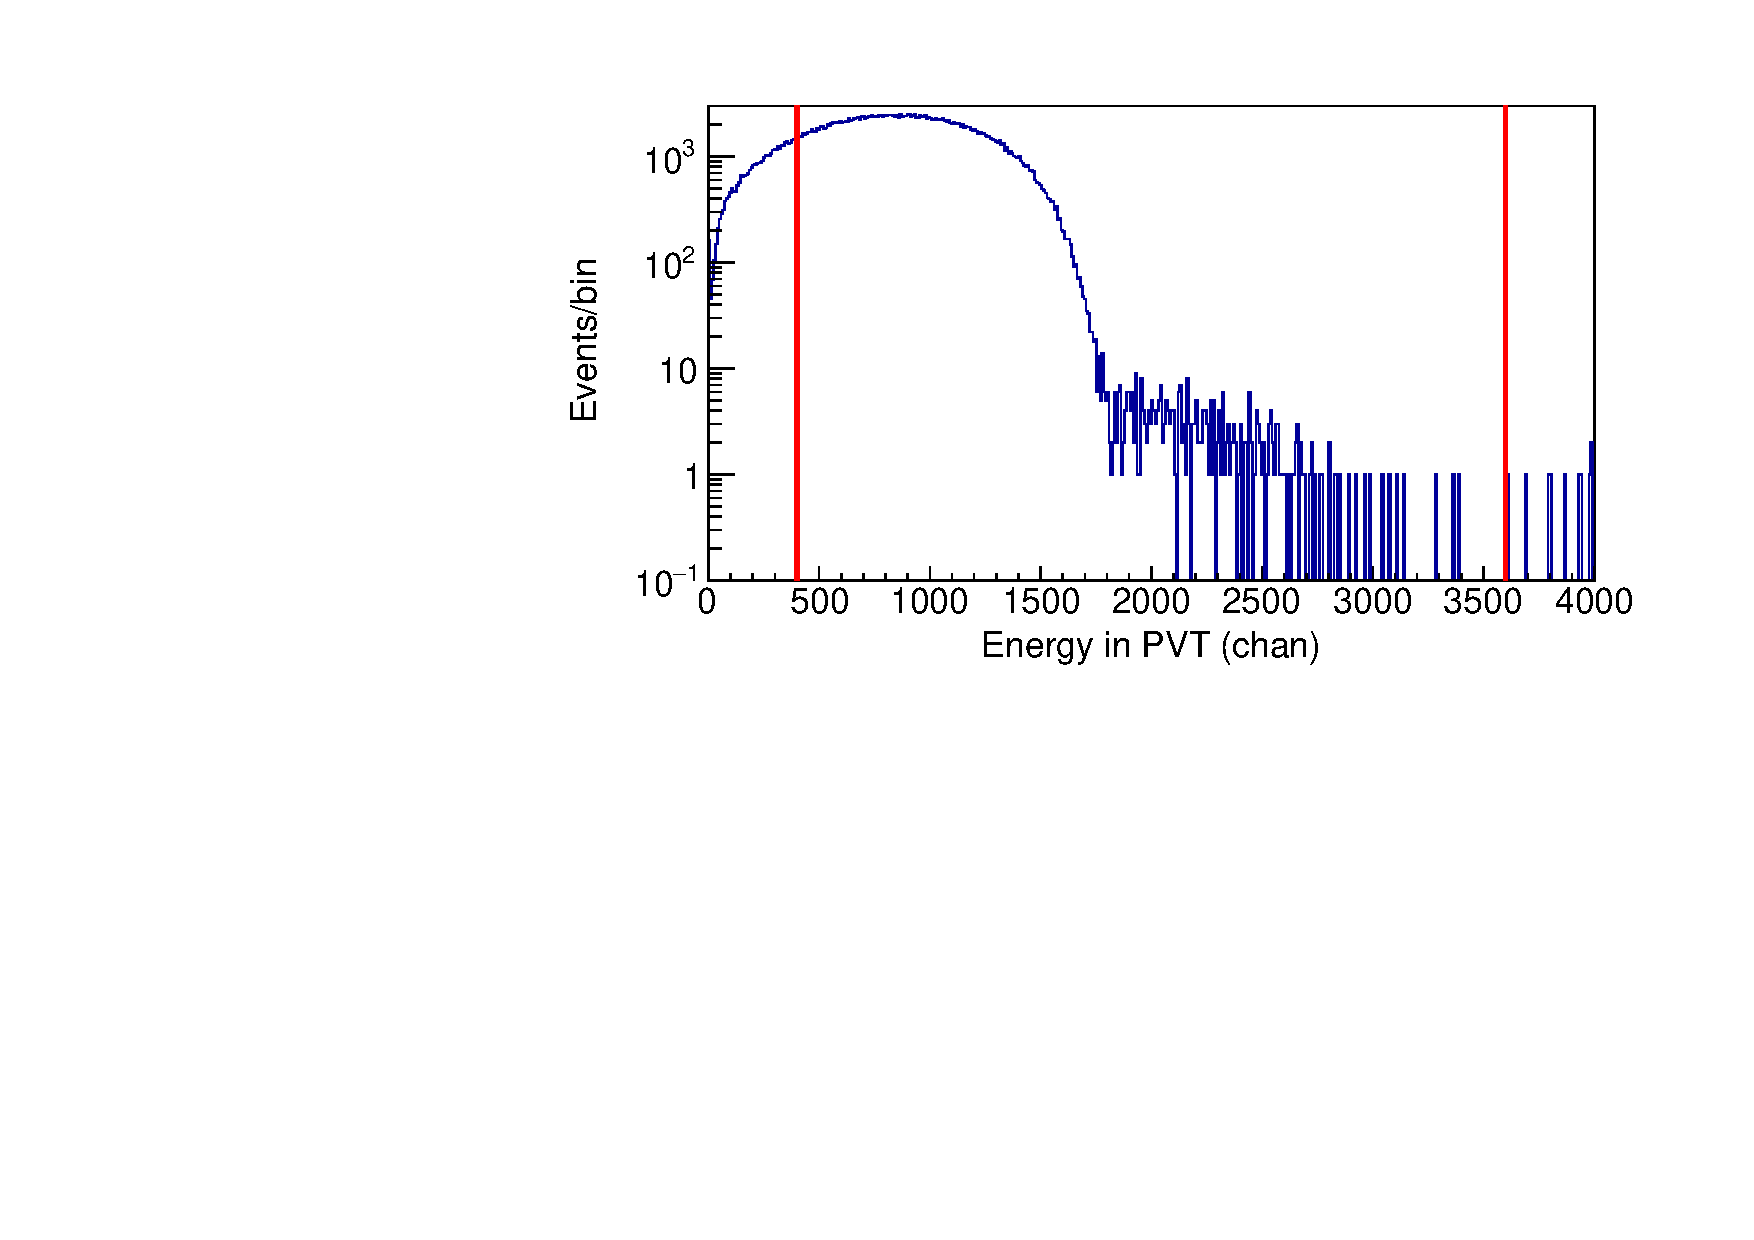
\includegraphics[width=0.78\textwidth]{fig_betaSpec.pdf}}
	\caption{
		 A beta spectrum built by applying the gamma cuts and time difference cuts. 
		 The beta cuts for the half-life analysis are shown as the red lines.
		 The lower beta cut was selected to be above the 511 region.
		 The upper beta cut was selected to include all the pile up}
	
	\label{fig:BetaGraph}
\end{figure}

\begin{figure}[!htb]
	\centerline{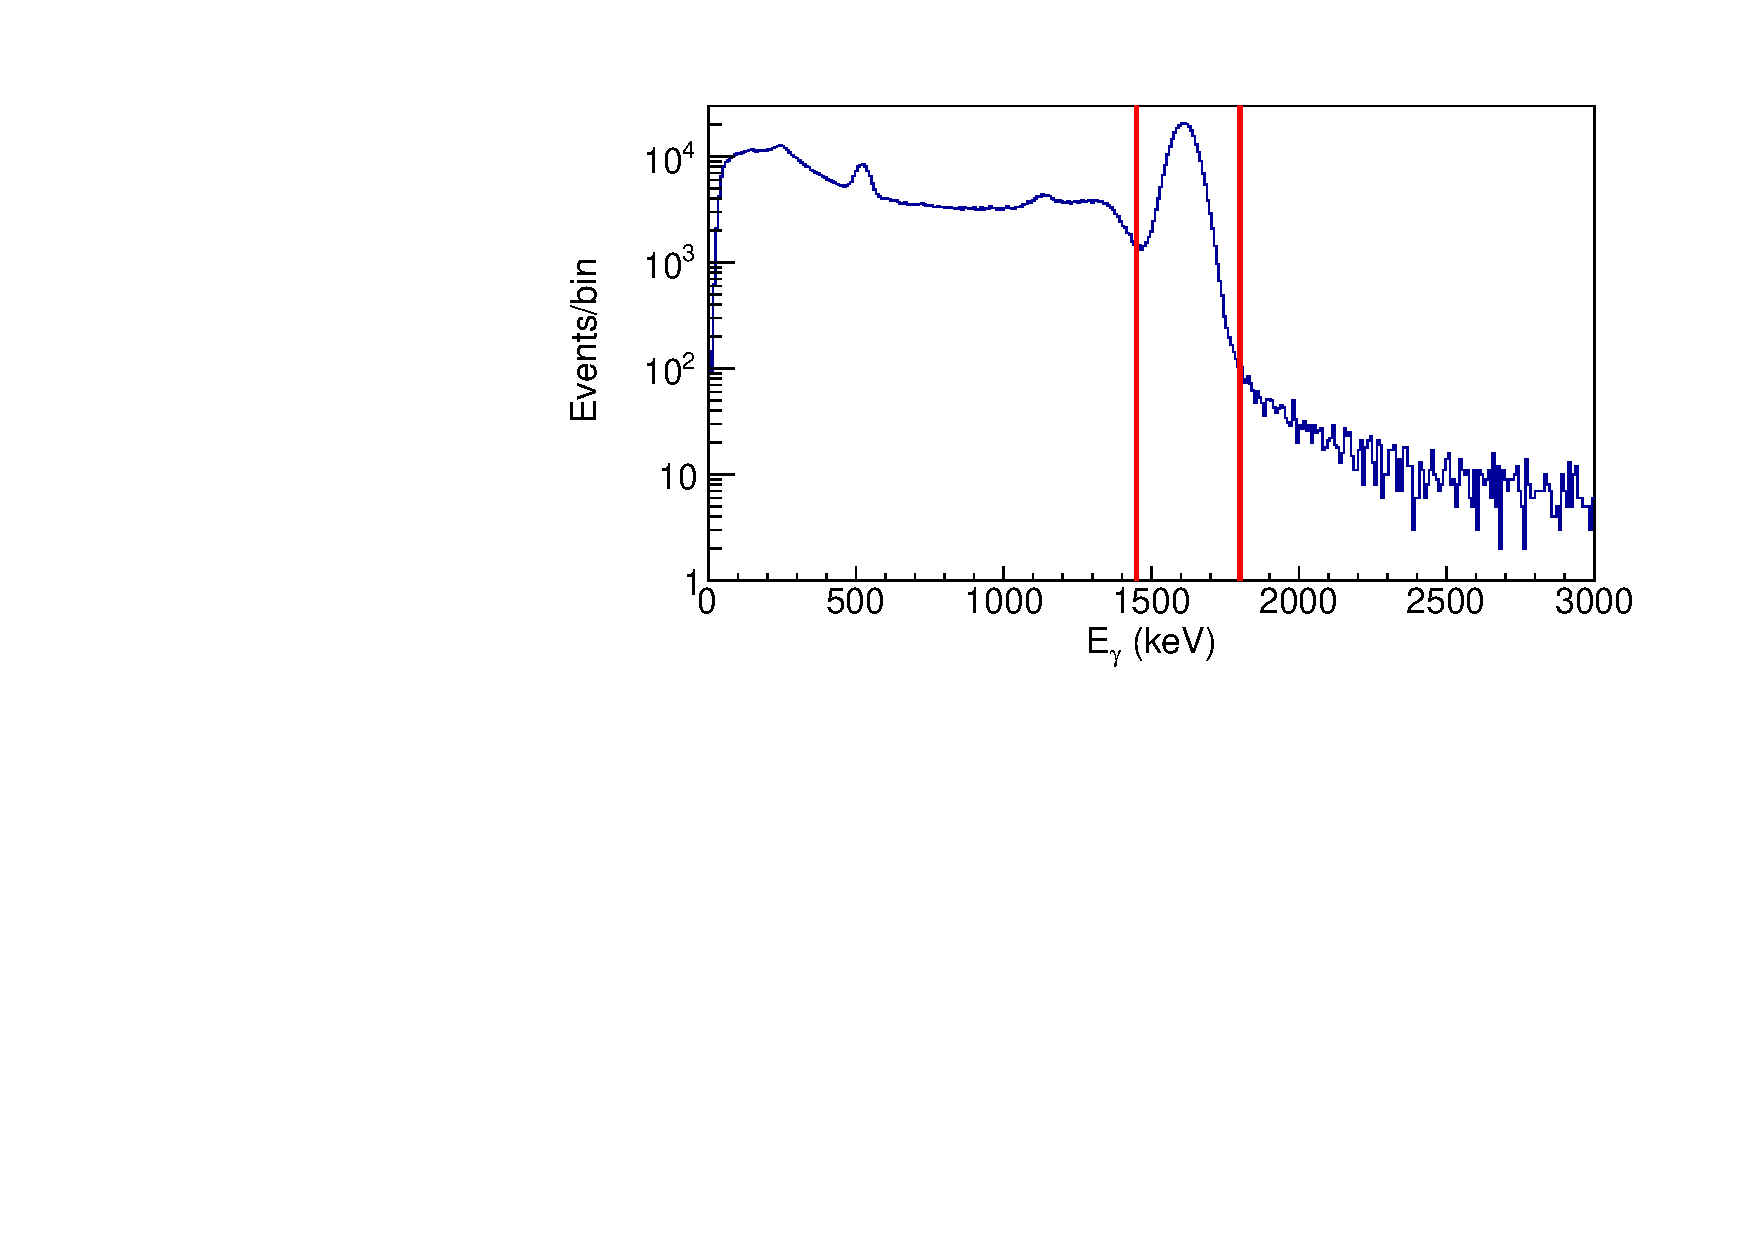
\includegraphics[width=0.78\textwidth]{fig_gammaSpec.pdf}}
	\caption{The wide cuts are to reduce the effect of the rate dependent gain.}
	\label{fig:GammaGraph}
\end{figure}

Fixed energy gates were used to select in the beta window for the PVT run sets.
Each different data set had a different energy window due to the gain shifts.
A sample spectrum with the gates can be seen in figure \ref{fig:BetaGraph}.
These cuts varied from set to set.
A summary of the PVT energy cuts can be seen in table \ref{tab:PVTCuts}.
This spectrum was put in coincidence with the gamma spectra. 
The lower beta cut was selected to cut out the 511 beta spectrum as seen in figure \ref{fig:2DGraph}.
When gated around that energies, the resulting gammas measured by the large CsI(Na) detectors are consistent with $^{10}$C and $^{11}$C.
This comes from the break-up of the $^{12}$C in the plastic scintillator. 

\begin{table}[!htb]
	\centering
	\caption{Energy cuts for the PVT detector}
	\begin{tabular}{lrr}
	Set & Lower Cut [ADC units] & Upper Cut [ADC units] \\ \hline
	1-2 & 2000 & 14400 \\
	3 & 1500 & 12000\\
	4 & 1700 & 13800 \\
	5 & 800 & 6200 \\
	6 & 480 & 4200 \\
	7 & 400 & 3600
	\end{tabular}
	\label{tab:PVTCuts}
\end{table}
As described above, only the runs after the installation of the limiter box were used for the half-life analysis. 
This would be sets 3-7.

A time difference condition was set by building a spectrum of the time differences between the implant detector's event and one of the four gamma detector's events. 
The peak of this time difference spectrum was found, and an interval of $\pm$24 ns  was use for this gate.
A sample time difference spectrum can be seen in figure \ref{fig:timediff}

\begin{figure}
	\centerline{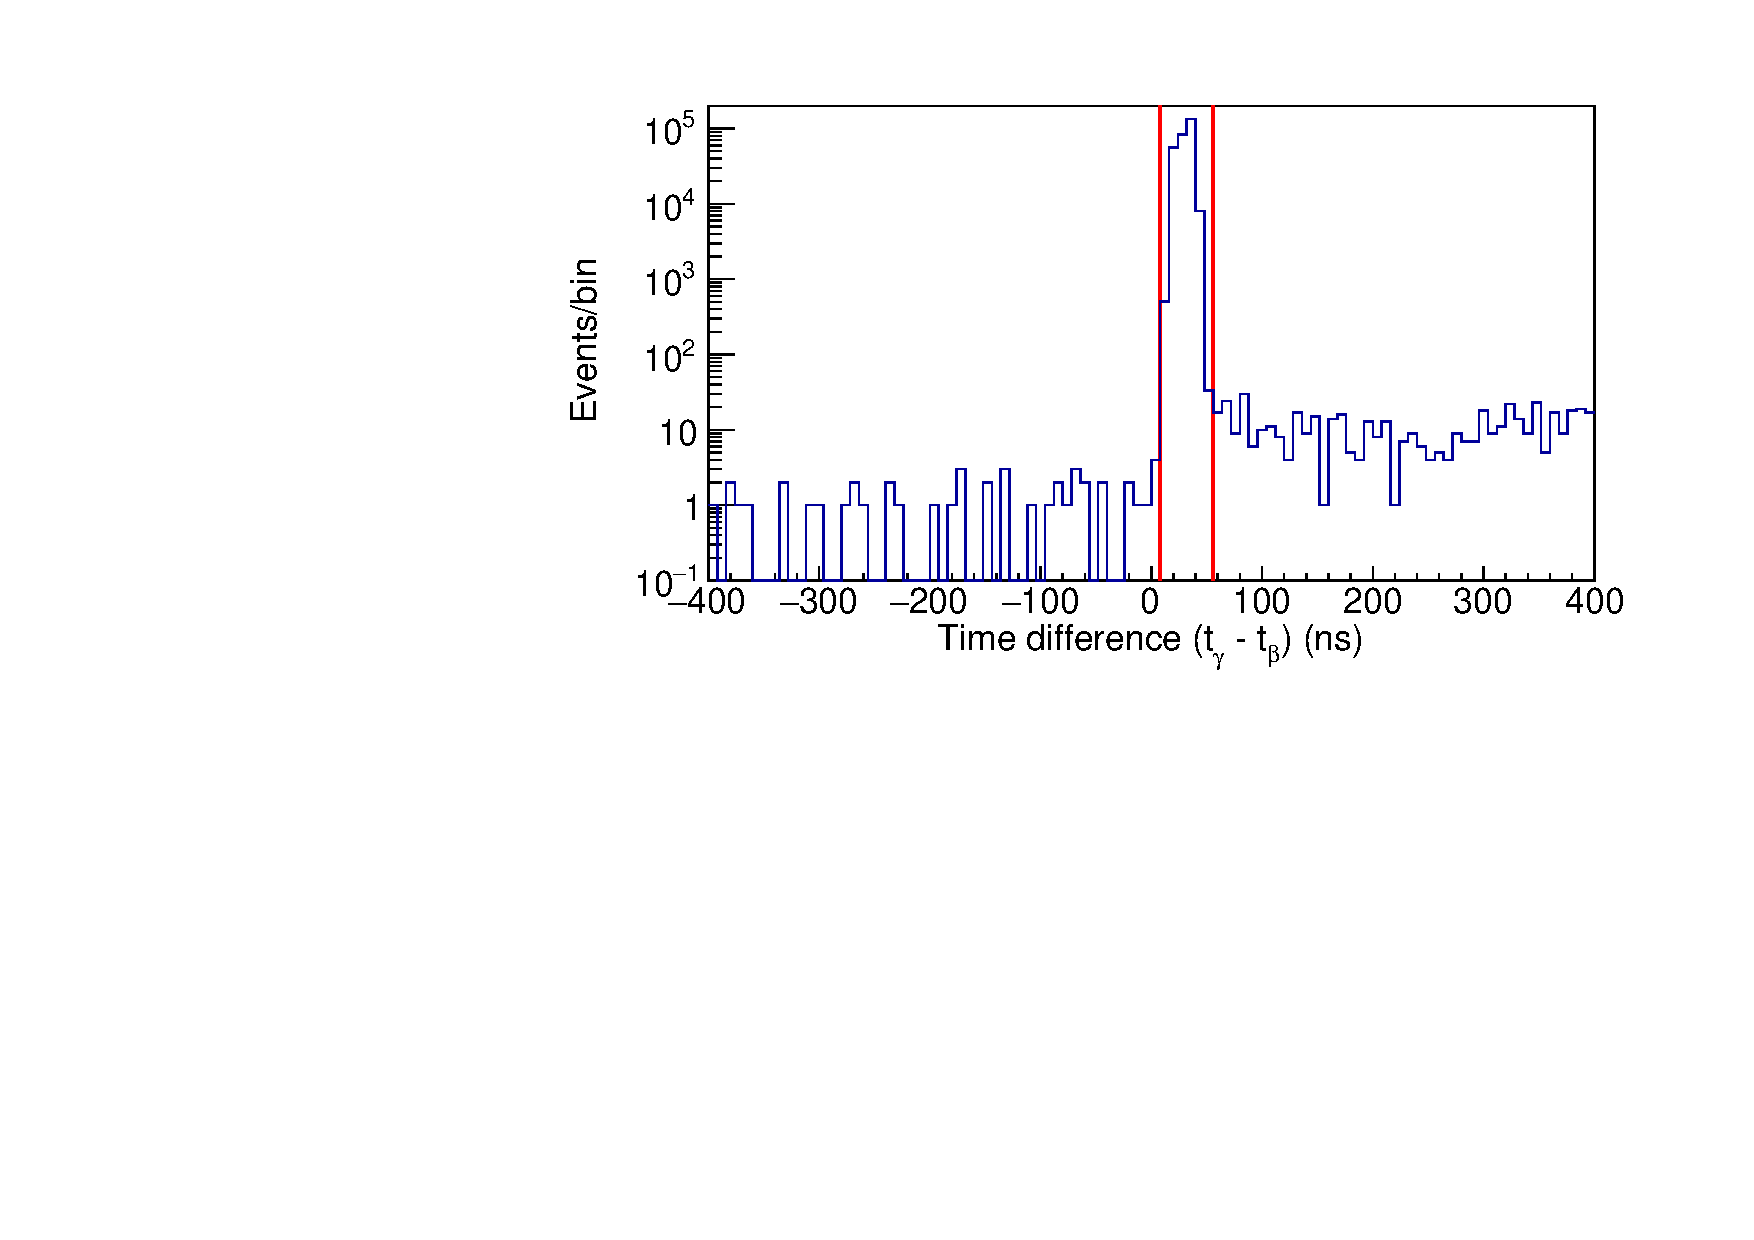
\includegraphics[width = 0.88\textwidth]{fig_tbgSpec1.pdf}}	
	\caption{The time difference between the up detector and the PVT implant detector.
		The tail on the right side of the large peak is due to pile up.
		The narrow time cuts are shown with a dotted line.
		The wide time cuts are shown with a solid line.}
	\label{fig:timediff}
\end{figure}

The time difference spectrum shows several features.
First is the prompt peak, which are correlated gamma and beta events. 
To the right of the prompt peak, there is a pedestal of events.
These come from pile-up events.
What happens is that a $^{20}$F event decays and the time stamp of the emitted beta is recorded.
The corresponding gamma ray is not detected.
Then, within the pile-up window, a second $^{20}$F decays.  
The implant detector is dead and does not record the second time stamp.
Due to pile-up, the time stamp of the second beta event is not recorded.
The gamma ray is then detected at a later time compared to the first event.
An cartoon sketch of this effect is shown in figure \ref{fig:PileUp}.
The pedistal can be seen in full in figure \ref{fig:timediff2}.

\begin{figure}
	\centerline{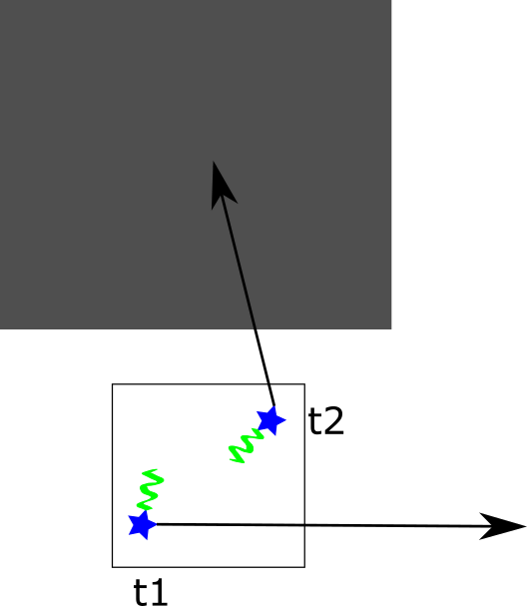
\includegraphics[width = 0.5\textwidth]{PileUpSketch.png}}
	\caption{A sketch of the pile up events.
		 A $^{20}$F decay happens at time = t1.
		 The green electron is detected in the implant detector.
		 The black arrow (the gamma raw) is not.
		 Then, later at time = t2, another $^{20}$F decays.
		 t2 is within the pile-up window of t1.
		 Both electrons energies pile-up and are added together.
		 However, the time stamp recorded by the DAQ is still t1.
		 The gamma ray from event t2 can be detected in a gamma detector at time t2.
		 This creates the uncorrelated event pedistal in the time difference graph.
		 }
	\label{fig:PileUp}
\end{figure}

\begin{figure}
	\centerline{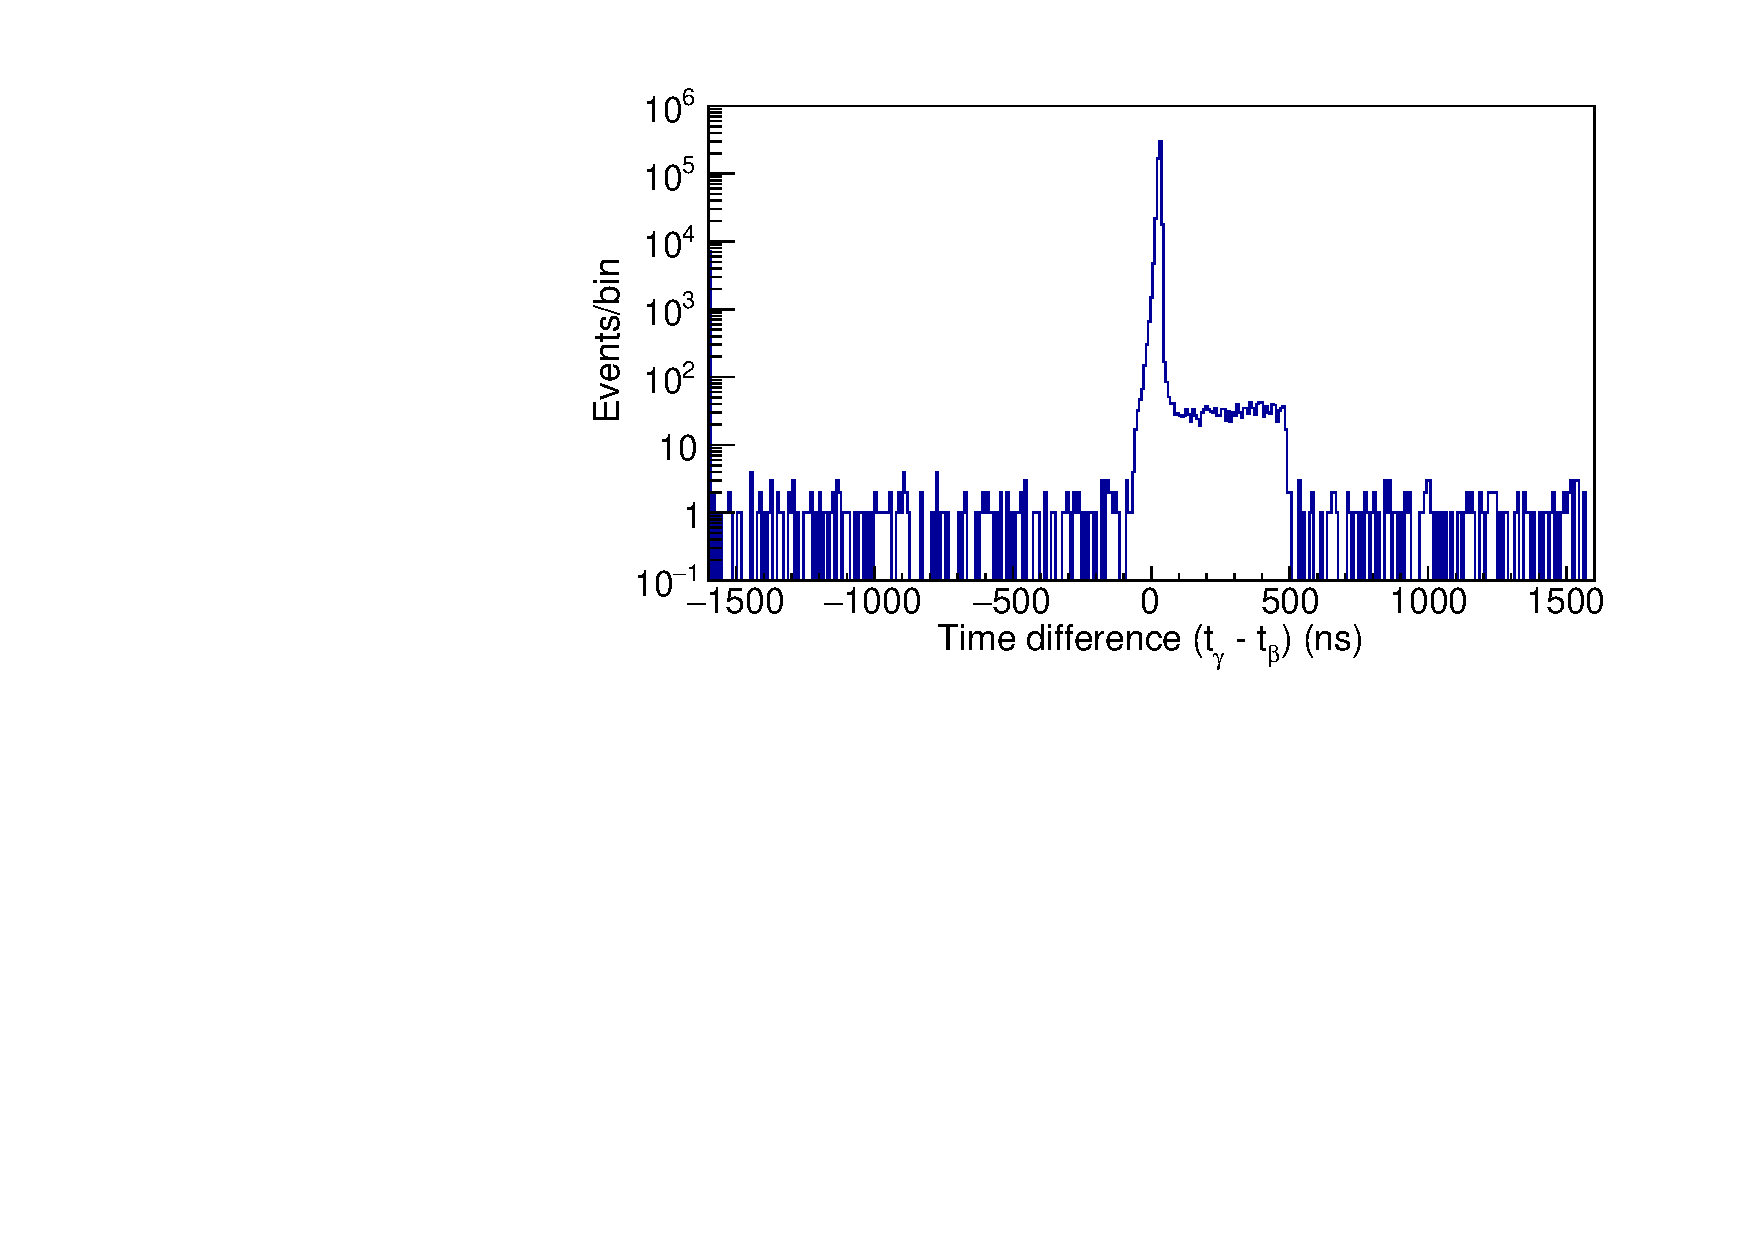
\includegraphics[width = 0.88\textwidth]{fig_tbgSpec2.pdf}}	
	\caption{The time difference spectrum zoomed out.
		 This figure is built from with energy coincidences with energy cuts.}
	\label{fig:timediff2}
\end{figure}

The other events to the left of the prompt peak and to the right of the pile-up pedestal are accidental coincidences.
These include the background coincidences.

The time signals for the outer four gamma detectors were used for the half-life analysis.
This gave 4 independent measurements of the half-life per run. 
Only full decay cycles were used. 
This was done by finding the last beam on and putting a condition on the run time of the events.

The dead time was corrected using measured rates and a dead time of 464 ns for the implant detector and 656 ns for the gamma detectors.  
The dead time was measured by building a spectrum of the time difference between consecutive time stamps.
The lowest time difference was taken as the dead  time. 
This was checked using the light pulser in the PVT detector.
For each gamma detector, a histogram of the energy-filtered rate was built.
The unfiltered implantation detector rate and gamma rate was built.
Using the uncorrected rates as an input, the gamma detector rate was corrected for bin by bin.
The correction used is 
%
\begin{equation}
r^{c}_{coincidence} = \frac{1}{1 - r_{\beta}\tau_{\beta}}\frac{1}{1 - r_{\gamma}\tau_{\gamma}}r^{m}_{coincidence} 
	\label{eq:dtc} 
\end{equation}
%
where $r^{c}_{coincidence}$ is the corrected gamma-beta coincidence rate, $r_{\beta}$ the raw measured implant rate, $\tau_{\beta}$ the dead time of the implant detector, $r_{\gamma}$ and $\tau_{\gamma}$ the raw measured rate and dead time for the CsI(Na) detector, and $r^{m}_{coincidence}$ the measured coincidence rate.   
Then, after corrected for the dead time, each cycle was added together relative to the last beam off.
These stacked cycles were used to find the half life.

For high beam intensity runs (i.e. sets 4,5 and 7), the dead-time corrections had a size of 31 to 36 ms.
For low beam intensity runs, (i.e. set 3) the dead-time correction changed the half-life by 6 to 8 ms. 
The values shown in this chapter are those with the dead-time correction.

Once the decay spectra were put in coincidence and stacked up, it was fit with the function
%
\begin{equation}
	f(t) = a\exp{(-t*ln2/T_{\frac{1}{2}})}
	\label{eq:fit-function}
\end{equation}
%
where $a$ and $T_{\frac{1}{2}}$ are free parameters.
$a$ is the initial rate and $T_{\frac{1}{2}}$ the half-life.
The decay curves were fit from 1.5 seconds past the beam on time to 1.5 second from the end of the decay time. 
The fitting method used was the log likelihood method. 
The 60 second decay run up detector result is shown in figure \ref{fig:60secdecay}.
From this run, it is seen that the spectra does not decay back down to the background. 
The lack of background parameter in equation \ref{eq:fit-function} comes from this observation. 

\begin{figure}[!htb]
\centerline{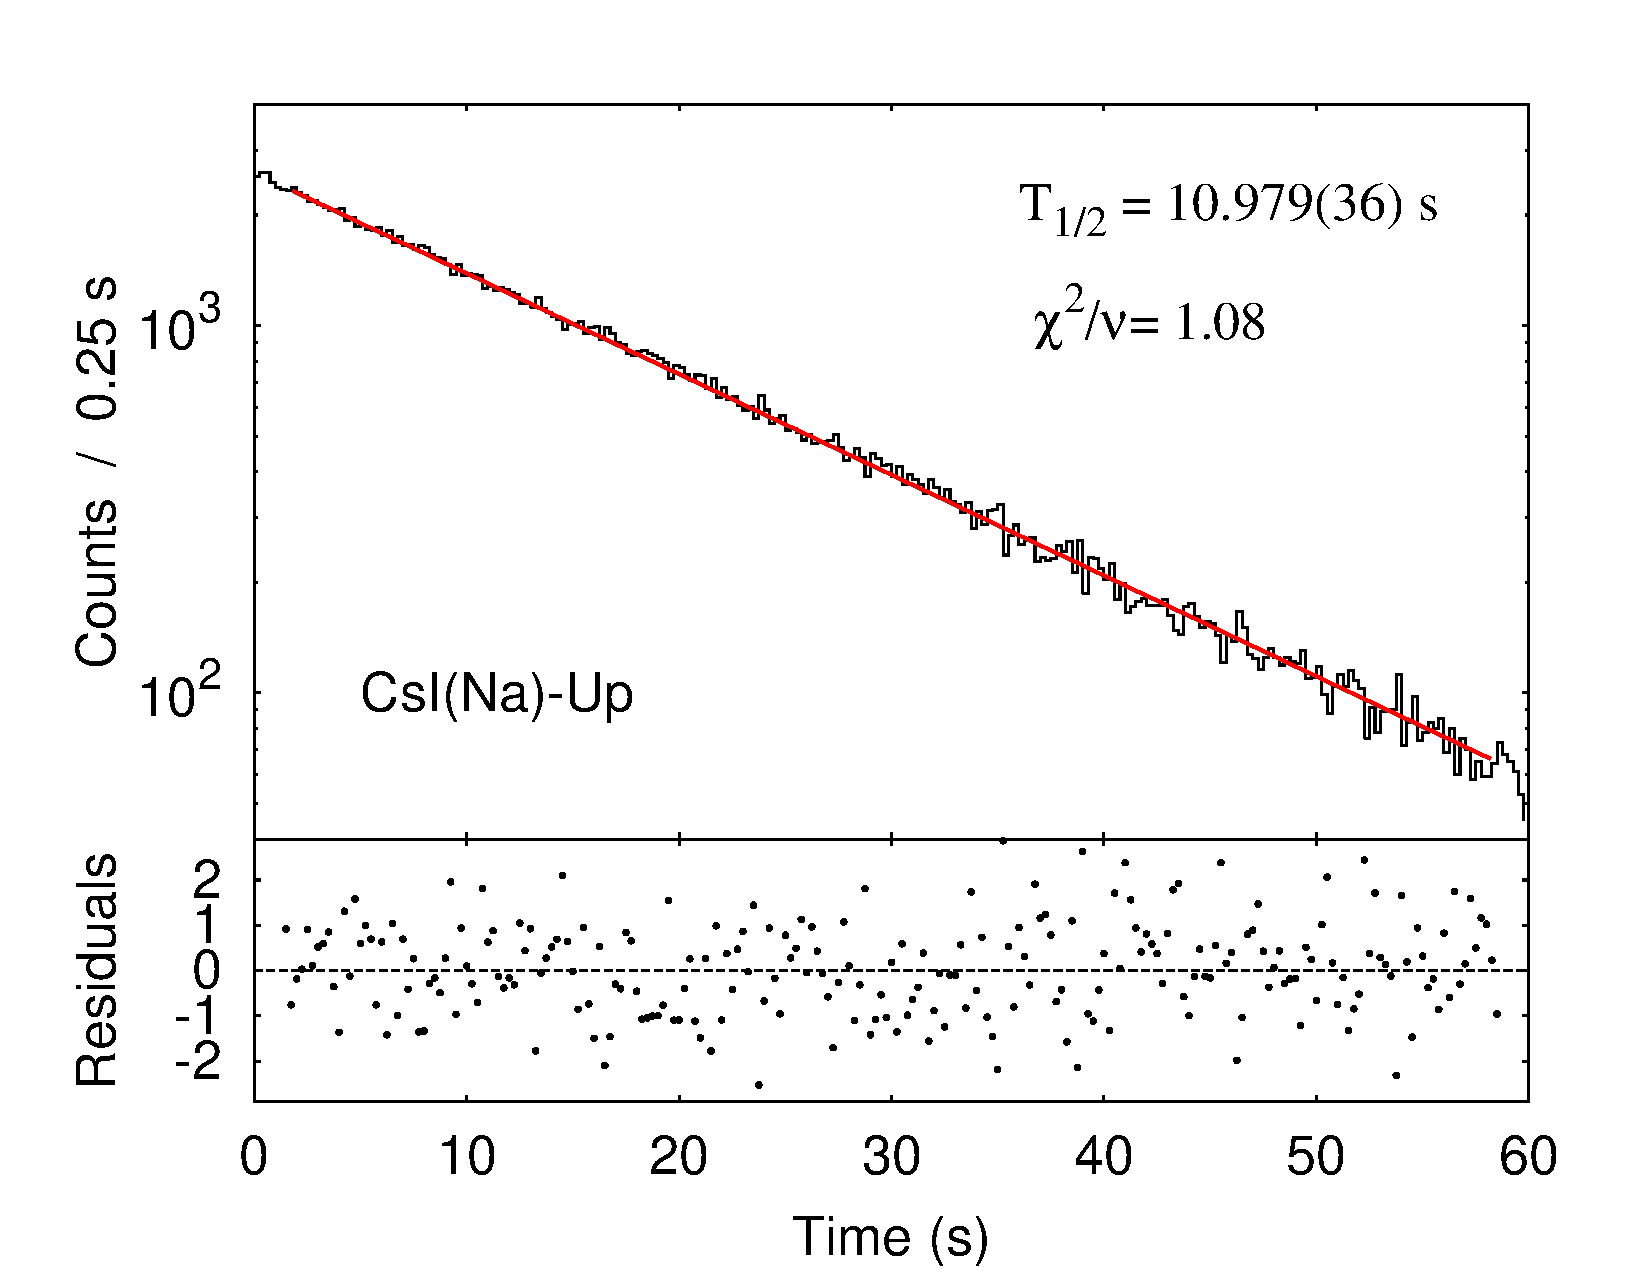
\includegraphics[width=0.88\textwidth]{fig_decaySpec.pdf}}
\caption{The decay spectrum from the up gamma detector is shown on the top graph.
	The red line is the exponential fit. 
	The bottom graph shows the residuals from the fit. 
	}
\label{fig:60secdecay}
\end{figure}


The decay spectra were built run by run, and the resulting fitting results were averaged together. 
Runs with a p-value less than 0.05 were considered statistically insignificant and thrown out.
After all the significant half-lives were collected, the average of them all was taken.

\section{Systematic Effects}
Several systematic effects were looked at.
The dead time correction was applied before any other systematics were investigated. 

\subsection{Dead Time}
The timing resultion of the clock is 8 ns.
Due to this, there is an uncertainty on the dead times of at least 8 ns.
The dead times were varied $\pm$4 ns and the half lives calculated.
Half the difference of those half lives is the systematic uncertainty.

\subsection{Pile-up Effects}
The dead time is over-corrected. 
Due to pile up, some of the pile up events are not totally lost.
Some of the events thought to be missing just got shuffled around.
This is a problem due to the fact that energy gates are imposed.
The pile-up events also have a different time structure than the regular events.
Due to the fact that the pile-up goes as the singles rate squared, the half-life of the pile-up events is half that of the non-piled-up events.
This creates a background with a different time signature, and causes a change in half-life.

The 48 ns time cut around the peak, shown in figure \ref{fig:timediff}, was compared to several other, larger time cuts.
The narrow time cut still has some uncorrelated background and pile-up events in them.


To account for this effect, several other time cuts were taken.
These cuts were plotted vs half-life in figure \ref{fig:timediffvhl}. .
The values were fit with a quadratic function.
This function was extrapolated to zero, which was the correction due to the pile-up.
 

\begin{figure}[!htb]
\centerline{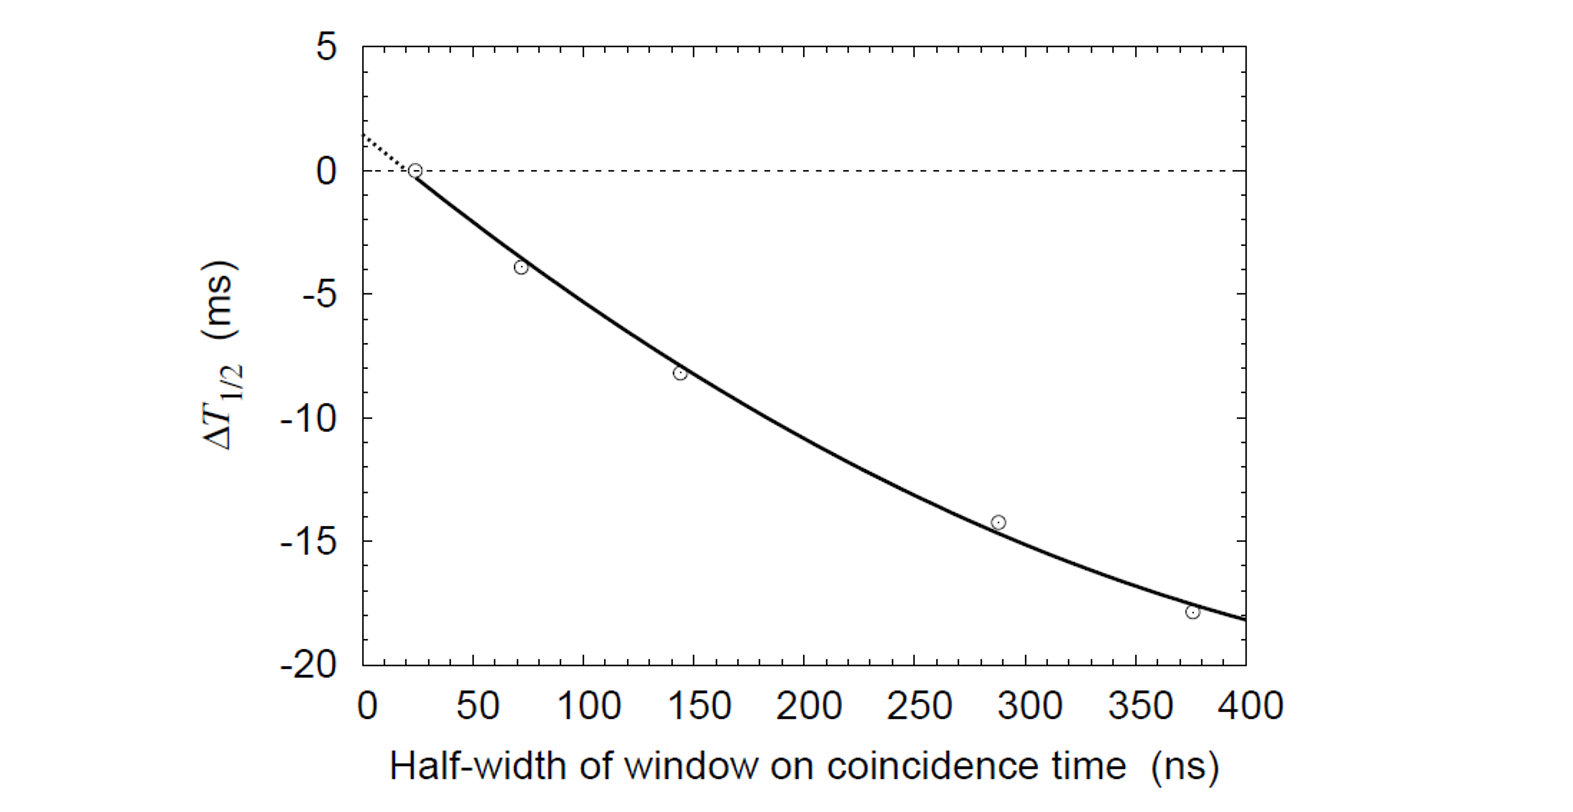
\includegraphics[width=0.88\textwidth]{fig_hlVsWtbg.png}}
\caption{Time difference vs the resulting half-life.
	 The line is a quadratic fit which was extrapolated to zero.
	}
\label{fig:timediffvhl}
\end{figure}
 
The extrapolation line is shown.
The half-life was corrected to the zero value of the window.
The difference between this extrapolated value and the previously measured value was taken as a correction and as an error bar.
 
\subsection{Background}

The first systematic effect is the effect of background.
Due to the low decay time, directly fitting a background is impossible.
There is no background region for the fitting function to anchor to, which induces a large correlation between the background and the half life.
Several techniques were used to estimate the background.

\subsubsection{Simultaneous vs Separate Fitting}
The first attempt was by simultaneously fitting each run with a different fitting function.
The equation used was 
%
\begin{equation}
	f(t) = a(\exp{-t*ln2/T_{\frac{1}{2}}} + b)
	\label{eq:fit-bg}
\end{equation}
%
with $b$ the relative background level.
The half-life of the four detectors was set to be a common parameter. 
The relative background level and initial rate, however, were assumed to be independent for each spectrum.
The resulting half life was compared to the value found with fitting each detector seperately without a background.

The effect of adding a background was investigated using Monte Carlo.
Exponential functions were generated and an amount of background added.
The resulting function was fit with a decay curve without a background parameter.
The amount of background added was varied, and the resulting half lives plotted.
It was found that increasing the background decreased the value of the half life, and that the background level and the half life value were strongly correlated.

A similar Monte Carlo was written to check the simultaneous fit method.
Four decay curves were simultaneously fitted the same way was the data.
They were also fitted separately with only an exponential decay.
The background was varied and the difference between the two values was taken.
The method shows a trend similar to the one seen in the previous Monte Carlo.

In the data, it was discovered that the results of the simultaneous vs separate fitting depended on the size of the dead time correction.
If the dead time was over-corrected, it induced an effect that was similar to having a larger background.
If more dead time was imposed, the effect was as if there was a negative background.
A dead time correction was added to the Monte Carlo, and a similar trend was seen.
As long as the dead time is known exactly, the background can be extracted with this technique. 

\subsubsection{Spectra Arguments}
The other way to try and gauge the background size is to look at the spectra.
Looking at figure \ref{fig:timediff}, it can be seen that on the left side of the large peak, there are very few counts.
It can also be seen that the prompt peak in the center contains most of the counts, while there is a long tail on the right side of the peak.
This tail is due to pile up. 
An event in the beta window piles up with another event later in time. 
The second event is read by a gamma detector, but is correlated with the first event, causing the large time difference.
The time spectrum changes if the beta spectrum is cut in different ways.

In the gamma beta 2D plot (figure \ref{fig:2DGraph}), it can be seen that there is no background events aside from the 511 region.
This is due to the presence of $^{10}$C and $^{11}$C.
When the detectors are put into tripple and quadruple coincidence, the gamma rays of those isotopes appear.
There are no gamma rays in the 1620 keV window which was filtered on..
The only coincidence possible is if there is pile up into that window along with a beta event.
The estimate of those events is shown on the left side of the peak in the time difference figure shown in figure \ref{fig:timediff}  
These events are accounted for when extrapolating the different time difference cuts, as shown in figure \ref{fig:timediffvhl}

\subsection{Cut Sensitivity}
For each pair of detectors, there were four conditions: two for each the implant and gamma detectors. 
For the gamma cuts, the edges of the gates were varied $\pm$ 5 keV in each direction for each cut.
The results is insensitive to the upper beta cut.
The lower beta cut was scanned with 6 different values going evenly from the initial lower beta cut to the peak of the spectrum.
Moving the lower beta cut also effects the dead time correction.
In order to disentangle the two, the lower beta cut was varied with two different time difference conditions.
The location where the difference between the two calculations blows up is where the effect of the lower beta cut starts being swamped by the effect of the pile up.
This is limit of where the lower beta cut was scanned.
All four of these conditions were varied independently, and the procedure of generation the spectrum and fitting the decay curves was done.
Half the resulting range of half-life values was taken to be a systematic uncertainty.
	
The fitting range of the decay spectra was varied. 
The start of the fit was varied bin by bin up to 6.5 seconds into the decay spectrum.
The end of the fit was varied the other way to cut out the end of the decay spectrum.
Since there was no noticeable systematic effect, there was no increase in error associated with this effect.

\subsection{Oscillator Stability}
The oscillator of the PIXE board has a stability of $\pm 5 * 10^{-5}$.
All times in the analysis were stretched by this value, and the half life calculated.
Have the difference between the stretched value and the original value is another systematic error.

\subsection{Binning and Fitting}
In order to check the sensitivity of the result to binning, the decay curves were rebinned by a factor of two.
Half the difference between the rebinned half life and the original half life is considered the correction and the uncertainty.

For the fitting method, log-likelihood estimators were used to fit the summed data.
This was done with two different packages which gave identical results. 
This was compared to analytic results, which gave the same results, so the half life is insensitive to the fitting method.

%%%%%%%%%%%%%%%%%%%%%%%%%%%%%%%%%%%%%%%%%%%%%%%%%%%%%%%%%%%%%%%%%%%%%%%%%%%%
\section{Result and Discussion}
\label{sec:result}

The half-lives obtained for all runs and all four detectors are shown in figure \ref{fig:PVT2by2}

\begin{figure}[!htb]
	\centerline{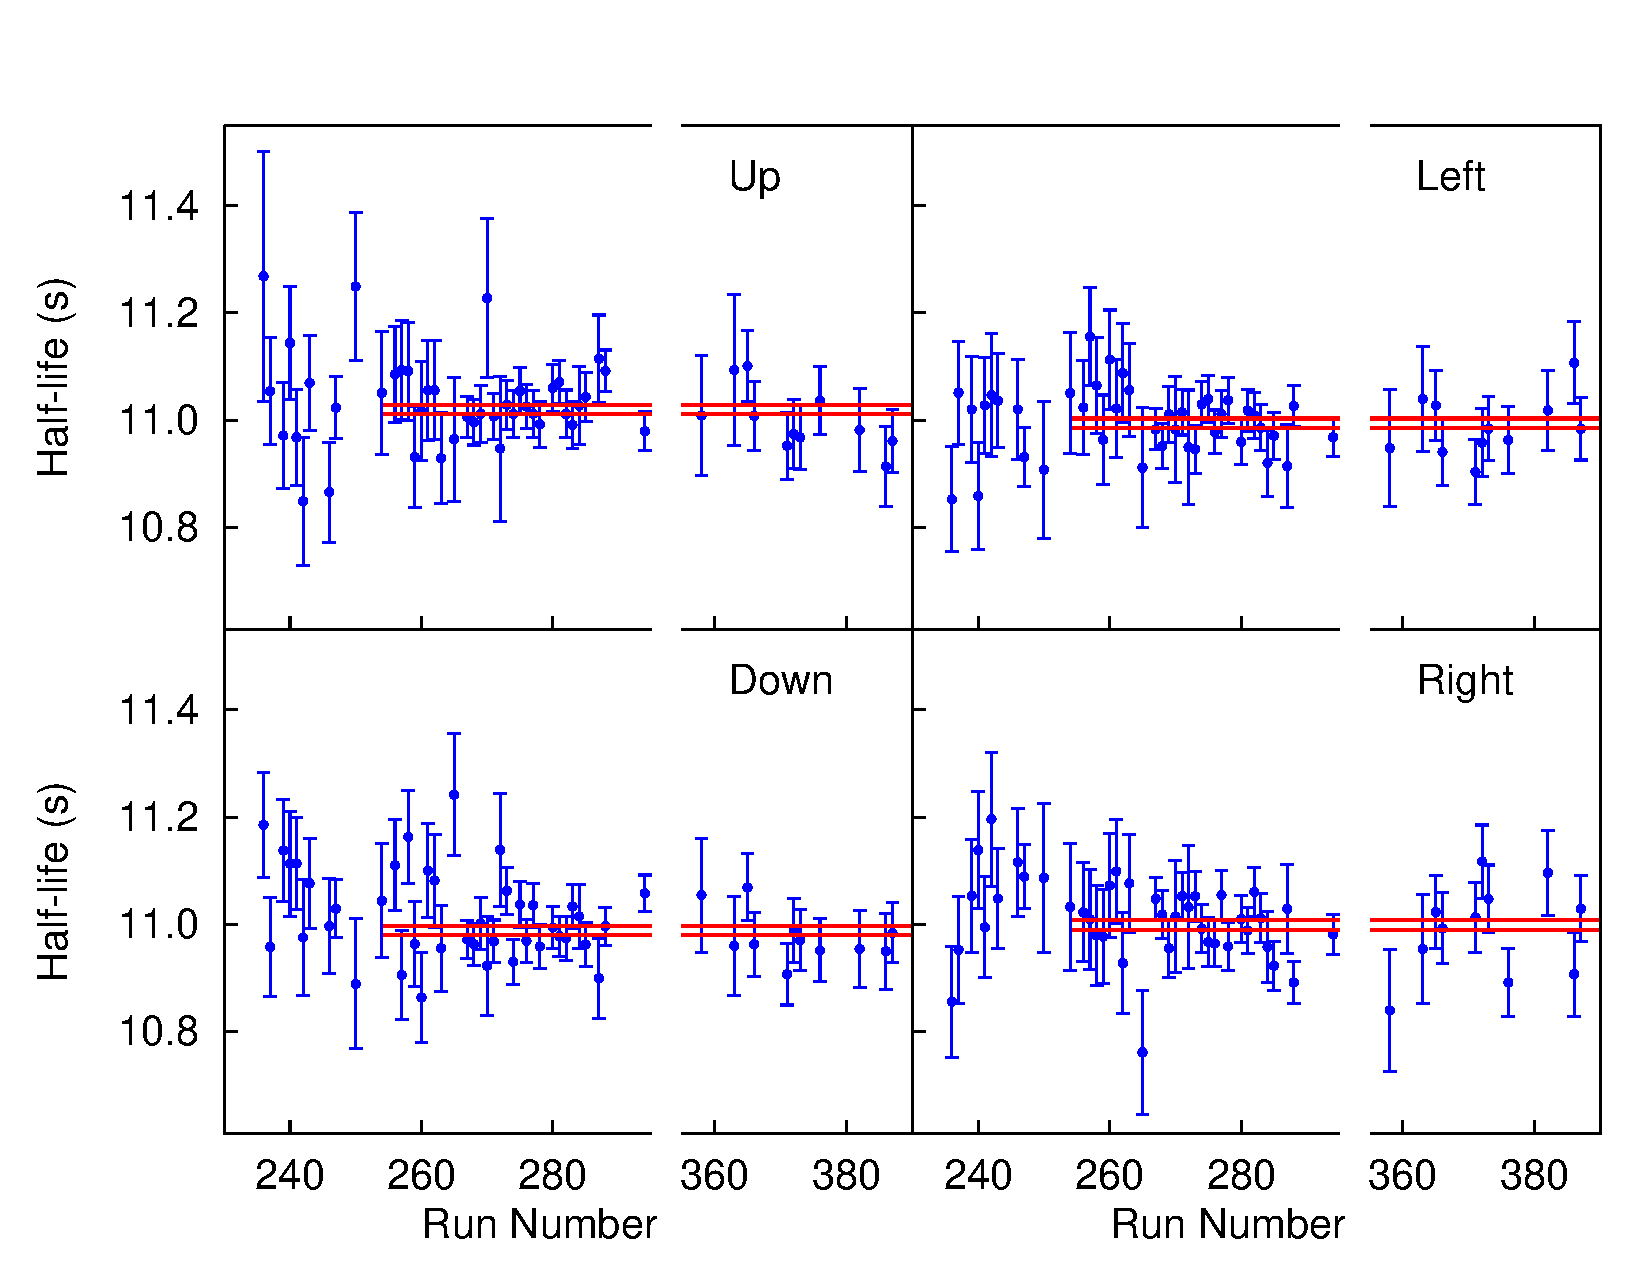
\includegraphics[width=0.88\textwidth]{fig_halfLives.pdf}}
	\caption{The red lines show the results of the fits over the runs that were used.
		 The additional half-lives shown are excluded to reasons discussed previously. 
		}
	\label{fig:PVT2by2}
\end{figure}

The results  are shown in  in table \ref{tab:PVTTable}.

%\begin{center}
	\begin{table}[!hbt]
			\centering
			\caption{Half-life results}
			\begin{tabular}{lrr}
			Detector & Half-Life & Error \\ \hline
			Up & 11.0195 & 0.0088 \\
			Left & 10.9944 & 0.0087 \\
			Down & 10.9980 & 0.0085 \\
			Right & 10.9987 & 0.0095 \\ 
			      &		& 	 \\
			Mean & 10.9999 & 0.0044
			\end{tabular}
			\label{tab:PVTTable}
	\end{table}
%\end{center}

The size of the systematic uncertainties investigated are shown in table \ref{tab:SysTable} 

%\begin{center}
\begin{table}[!hbt]
	\caption{Systematics}
	\centering
	\label{tab:err-budget}
		\begin{tabular}{lrr}
		Source & Correction [ms] & Uncertainty [ms] \\ \hline
		Dead-time & 0.00 & 0.24 \\
		Oscillator stability & 0.00 & 0.80 \\
		Lower PVT cut & 0.00 & 2.32 \\
		Lower gamma cut & 0.00 &  0.15\\
		Upper gamma cut  & 0.00 & 0.05 \\ 
		Uncorrelated events & 1.47 & 1.47 \\
		Binning & -0.30 & 0.30 \\
			&	&	\\
		Total systematic & 1.17 & 2.89
		\end{tabular}
	\label{tab:SysTable}
\end{table}
%\end{center}
After the dead time correction, the value of the half-life was found to be 11.0011 $\pm$ 0.0069 (stat) $\pm$ 0.0030 (syst) s.

%%%%%%%%%%%%%%%%%%%%%%%%%%%%%%%%%%%%%%%%%%%%%%%%%%%%%%%%%%%%%%%%%%%%%%%%%%%%
\section{Conclusion}
\label{sec:conclusion}

The half-life measured is most consistent with some previous measurements of a half-life of about 11 s. 
This can be seen in figure \ref{fig:ideogramfinal}.
This measurement disagrees with the most recent measurements.

\begin{figure}[!htb]
\centerline{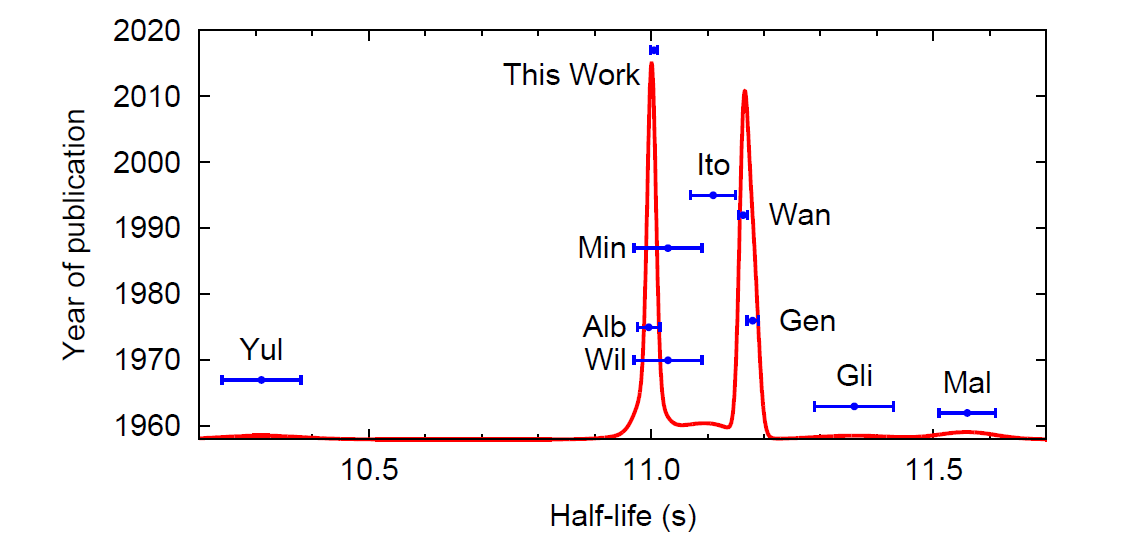
\includegraphics[width=0.88\textwidth]{fig_ideogramAfter.png}}
\caption{A scatter plot of previous values with this work added.
	 The labels correspond to: Mal~\cite{Mal62}, Gli~\cite{Gli63},
	Yul~\cite{Yul67}, Wil~\cite{Wil70}, Alb~\cite{Alb75}, Gen~\cite{Gen76},
	Min \cite{Min87}, Wan~\cite{Wan92} and Ito~\cite{Ito95}.}
\label{fig:ideogramfinal}
\end{figure}

Motivated by this measurement, another measure of the $^{20}$F half-life has been done. 
The outcome of the measurements was a half-life of 11.0160 (41)$_{stat}$(155)$_{sys}$ s \cite{Bur19}.
This confirms the result obtained in this measurement.

Several things about the data set were discovered.
It was learned that there were contaminates coming from the fragmentation of the $^{12}$C in the plastic scintillator.
It was also discovered that the rate dependent gain effect in the CsI(Na) implant detector is significant.
Before doing this measurement, it was assumed that the low rates would make that effect negligible.
It was learned that after the coincidence, the amount of background left in the spectrum is negligible, and that we have no contaminates in the beam.

\end{document}
%%%%%%%%%%%%%%%%%%%%%%%%%%%%%%%%%%%%%%%%%%%%%%%%%%%%%%%%%%%%%%%%%%%%%%%%%%%%
%Bibliography

%%%%%%%%%%%%%%%%%%%%%%%%%%%%%%%%%%%%%%%%%%%%%%%%%%%%%%%%%%%%%%%%%%%%%%%%%%%%
%%%%%%%%%%%%%%%%%%%%%%%%%%%%%%%%%%%%%%%%%%%%%%%%%%%%%%%%%%%%%%%%%%%%%%%%%%%%
